%%%%%%%%%%%%%%%%%%%%%%%%%%%%%%%%%%%%%%%%%%%%%%%%%%%%%%%%%%%%%%%%%%%%%%%
% BAB 4
%%%%%%%%%%%%%%%%%%%%%%%%%%%%%%%%%%%%%%%%%%%%%%%%%%%%%%%%%%%%%%%%%%%%%%%

\mychapter{4}{BAB 4 REKAYASA KEBUTUHAN}

\section{Deskripsi Umum Sistem}

Sistem yang dikembangkan pada penelitian ini adalah sistem pencegah
plagiarisme dengan menggunakan metode \emph{snapshotting} dan
\emph{user activity logging}. Sistem ini dibangun dengan tujuan untuk
meminimalisir adanya tindak plagiarisme. Sistem ini dibagi menjadi dua
bagian, pertama yaitu \emph{Lupv} (\emph{Lup Viewer}) yang digunakan
oleh dosen untuk membaca hasil rekaman yang dilakukan oleh sistem
kedua. \emph{Lupr} hanya dapat membaca berkas tugas yang berbentuk \emph{plain
  text format}. Sistem kedua yaitu \emph{Lupr} (\emph{Lup Recorder}), sistem
ini digunakan untuk merekam perubahan tugas dan aktivitas siswa selama
pengerjaan tugas berlangsung. \emph{Lupv} digunakan oleh dosen
sedangkan \emph{Lupr} digunakan oleh mahasiswa.

\emph{Lupv} memiliki beberapa fungsionalitas, di antaranya menampilkan
seluruh daftar rekaman, melihat aktivitas yang dilakukan selama
pengerjaan, dan melihat perubahan berkas tugas dari waktu ke
waktu. Di lain sisi, \emph{Lupr} memiliki fungsionalitas di antaranya
adalah merekam perubahan berkas tugas, alamat \emph{IP}, \emph{login
  name}, \emph{device name}, seluruh \emph{window} dan \emph{window} yang aktif.

Cara kerja sistem ini dimulai dengan mahasiswa yang menjalankan
\emph{Lupr} pada berkas tugas yang diberikan dosen. Setelah tugas
selesai dikerjakan, maka berkas tersebut kemudian dikirimkan ke dosen
yang bersangkutan. Dosen yang bersangkutan kemudian dapat melihat
seluruh hasil rekaman menggunakan \emph{Lupv}.


\begin{figure}[tph]
  \centering
  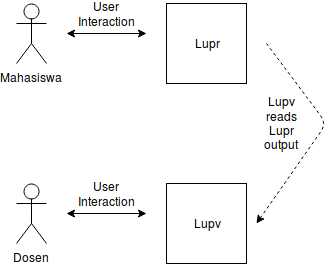
\includegraphics[width=.59\linewidth]{img/deskripsi-sistem}
  \caption{Gambaran umum sistem}\label{fig:deskripsi-sistem}
\end{figure}


\section{Analisis Kebutuhan}

Analisis kebutuhan pada sistem ini didapatkan dari beberapa sumber. Sumber
pertama adalah metode penelitian yang telah dilakukan oleh
\textcite{hellas2017plagiarism}. Sumber kedua didapatkan dari ``\emph{future
  work}'' penelitian \textcite{hellas2017plagiarism} dan penelitian
\textcite{leung2017instructional}. Penelitian \textcite{leung2017instructional}
memaparkan cara-cara plagiarisme di mana cara-cara tersebut belum dapat
ditangani oleh metode penelitian yang telah dilakukan
\textcite{hellas2017plagiarism}. Sumber kebutuhan ketiga adalah kelemahan dari
penelitian \textcite{hellas2017plagiarism} yang akan disempurnakan. Ketiga
sumber tersebut menghasilkan kebutuhan-kebutuhan pokok sistem yaitu
mengimplementasikan metode \emph{snapshotting} untuk merekam perubahan berkas,
metode \emph{user activity logging} untuk merekam aktivitas siswa saat
mengerjakan tugas, serta membangun sistem dengan sifat \emph{agnostic} agar
tidak terikat dengan \emph{platform} tertentu.

Sistem yang dikembangkan memiliki batasan hanya dapat berjalan pada
sistem operasi \emph{GNU/Linux}. Terdapat banyak \emph{desktop
  environment} yang ada pada sistem operasi \emph{GNU/Linux}. Maka
sistem harus dapat berjalan dengan baik pada berbagai macam
\emph{desktop enviroment} yang memiliki format nama \emph{window} yang
berbeda-beda. Oleh karena itu, kebutuhan non-fungsional yang harus
dimiliki oleh sistem adalah \emph{compatibility} sistem pada berbagai
macam \emph{desktop environments}. Jumlah \emph{desktop environment}
yang tidak terbatas membuat penelitian ini membatasi jumlah
\emph{desktop environment} yang didukung. \emph{Desktop environment}
yang didukung terbatas pada enam \emph{desktop environment} yang umum
digunakan, yaitu \emph{GNOME, KDE, XFCE, Unity, Cinnamon} dan
\emph{Phanteon}.

\section{Identifikasi Aktor}


Berdasarkan proses analisis kebutuhan yang dilakukan, terdapat satu
aktor utama pada sistem \emph{Lup Viewer} yaitu dosen, dan satu aktor utama
pada sistem \emph{Lup Recorder} yaitu mahasiswa. Tabel~\ref{tab:aktor-lupv} memaparkan daftar aktor yang
terlibat dalam sistem \emph{Lup Viewer} beserta deskripsinya, dan
Tabel~\ref{tab:aktor-lupr} memaparkan daftar aktor yang terlibat
pada sistem \emph{Lup Recorder} beserta deskripsinya.

{\makegapedcells
  \begin{longtable}{|c|L{2cm}|L{9cm}|}
   \caption{Identifikasi aktor pada sistem \emph{Lup Viewer}}\label{tab:aktor-lupv}\\
    \hline
    \thead{No} & \thead{Aktor} & \thead{Deskirpsi}\\\hline
    \endfirsthead
    \hline
    \thead{No} & \thead{Aktor} & \thead{Deskirpsi}\\\hline
    \endhead
    1 & Dosen & Dosen merupakan suatu individu atau kelompok
                yang berperan dalam memberikan tugas dan
                menganalisis hasil tugas yang telah dikerjakan oleh
                mahasiswa. \\\hline
  \end{longtable}
}

{\makegapedcells
  \begin{longtable}{|c|L{2cm}|L{9cm}|}
    \caption{Identifikasi aktor pada sistem \emph{Lup Recorder}}\label{tab:aktor-lupr}\\
    \hline
    \thead{No} & \thead{Aktor} & \thead{Deskirpsi}\\\hline
    %
    1 & Mahasiswa & Mahasiswa merupakan suatu individu atau
                    kelompok yang berperan dalam mengerjakan tugas yang
                    diberikan oleh dosen.\\\hline
  \end{longtable}
}

\section{Kebutuhan Fungsional Sistem}

Kebutuhan fungsional merupakan sebuah kebutuhan yang harus disediakan
oleh sistem, bagaimana sistem bereaksi terhadap suatu masukan, dan
bagaimana sistem berperilaku pada suatu
keadaan~\parencite{sommerville2016software}. Daftar kebutuhan
fungsional didapatkan dari proses analisis kebutuhan yang telah
dilakukan sebelumnya. Dalam penelitian ini, kebutuhan fungsional
memiliki sistem penomoran LUPV-F-XX-YY untuk sistem \emph{Lup Viewer}
dan LUPR-F-XX-YY untuk sistem \emph{Lup Recorder}. \emph{LUPV} dan
\emph{LUPR} merupakan nama sistem, F menunjukkan tipe kebutuhan yaitu
kebutuhan fungsional, XX menunjukkan nomor kebutuhan, dan YY
menunjukkan nomor spesifikasi
kebutuhan. Tabel~\ref{tab:kebutuhan-fungsional-lupr} dan
Tabel~\ref{tab:kebutuhan-fungsional-lupv} memaparkan daftar kebutuhan
fungsional, beserta definisi, aktor yang terlibat, dan pemetaan nama
\emph{use case} yang didapatkan dari hasil analisis kebutuhan untuk
sistem \emph{Lup Recorder} dan \emph{Lup Viewer}.


{\makegapedcells
  \begin{longtable}{|c|L{2.5cm}|L{5cm}|L{1.8cm}|L{2.1cm}|}
    \caption{Spesifikasi kebutuhan fungsional, definisi, dan pemetaan nama \emph{use case} sistem \emph{Lup Recorder}}
    \label{tab:kebutuhan-fungsional-lupr}\\\hline
    \thead{No} & \thead{Kode\\ Kebutuhan} & \thead{Deskripsi Kebutuhan}
                                          &  \thead{Aktor} & \thead{Nama \\ \emph{Use Case}} \\\hline
    \endfirsthead
    \hline
    \thead{No} & \thead{Kode\\ Kebutuhan} & \thead{Deskripsi Kebutuhan}
                                          &  \thead{Aktor} & \thead{Nama \\ \emph{Use Case}} \\\hline
    \endhead\hline\endfoot
    %
    1 & LUPR-F-01 & Sistem harus menyediakan fungsi untuk merekam
                    pengerjaan tugas. & Mahasiswa & Merekam pengerjaan
                                                    tugas. \\\cline{1-3}
    1.1 & LUPR-F-01-01 & Sistem harus menyediakan tombol ``\emph{Start
                         Recording}'' sebagai sarana untuk menjalankan
                         perekaman tugas. &  & \\\cline{1-3}
    1.2 & LUPR-F-01-02 & Sistem harus menyediakan fungsi untuk memilih
                         direktori tempat tugas dikerjakan. & & \\\cline{1-3}
    1.3 & LUPR-F-01-03 & Data yang harus direkam adalah berkas tugas,
                         alamat \emph{IP}, seluruh \emph{window},
                         \emph{window} yang aktif, nama \emph{login}, dan
                         nama piranti. & &\\\cline{1-3}
    1.4 & LUPR-F-01-04 & Sistem harus menampilkan notifikasi ``\emph{Lup is recording}'' ketika
                         perekaman mulai berjalan. & & \\\cline{1-3}
    1.5 & LUPR-F-01-05 & Sistem harus menyediakan tombol ``\emph{Stop and
                         Quit}'' sebagai sarana untuk menghentikan
                         perekaman tugas dan keluar dari sistem.  & & \\\hline
    2 & LUPR-F-02 & Sistem harus menyediakan fungsi untuk mengubah
                    nilai interval rekaman. & Mahasiswa & Mengubah
                                                          interval
                                                          rekaman. \\\cline{1-3}
    2.1 & LUPR-F-02-01 & Sistem harus menyediakan tombol ``\emph{Set
                         Interval}'' sebagai sarana untuk mengubah
                         interval rekaman. & & \\\cline{1-3}
    2.2 & LUPR-F-02-02 & Sistem harus menyediakan kolom dialog untuk
                         mengisi nilai interval. & & \\\cline{1-3}
    2.3 & LUPR-F-02-03 & Nilai interval hanya dapat diisi angka
                         bilangan bulat diatas 0.  & & \\\cline{1-3}
    2.4 & LUPR-F-02-04 & Sistem harus menampilkan peringatan ``\emph{Interval must higher than 0}'' jika
                         kolom interval diisi dengan selain bilangan bulat diatas 0.& & \\\cline{1-3}
    2.5 & LUPR-F-02-05 & Sistem harus menonaktifkan tombol ``\emph{Set Interval}'' ketika perekaman belum
                         dijalankan. & & \\\cline{1-3}
    2.6 & LUPR-F-02-06 & Sistem harus menampilkan notifikasi ``\emph{Interval changed to <<nilai
                         interval>>}'' ketika nilai interval berhasil dirubah.  & & \\\hline
  \end{longtable}
}

{\makegapedcells
  \begin{longtable}{|c|L{2.5cm}|L{5cm}|L{1.8cm}|L{2.1cm}|}
    \caption{Spesifikasi kebutuhan fungsional, definisi, dan pemetaan nama \emph{use case} sistem \emph{Lup Viewer}}
    \label{tab:kebutuhan-fungsional-lupv}\\\hline
    \thead{No} & \thead{Kode\\ Kebutuhan} & \thead{Definisi Kebutuhan}
                                          &  \thead{Aktor} &  \thead{Nama\\ \emph{Use Case}}\\\hline
    \endfirsthead
    \hline
    \thead{No} & \thead{Kode\\ Kebutuhan} & \thead{Definisi Kebutuhan}
                                          &  \thead{Aktor} &  \thead{Nama\\ \emph{Use Case}}\\\hline
    \endhead\hline\endfoot
    %
    1 & LUPV-F-01 & Sistem harus menyediakan fungsi untuk menampilkan
                    seluruh daftar rekaman mahasiswa. & Dosen & Melihat seluruh
                                                                daftar rekaman. \\\cline{1-3}
    1.1 & LUPV-F-01-01 & Sistem harus menyediakan tombol ``\emph{Open Records}''
                         sebagai sarana untuk memilih rekaman yang akan
                         ditampilkan. & & \\\cline{1-3}
    1.2 & LUPV-F-01-02 & Sistem hanya dapat membaca direktori dengan
                         format ``<<namamahasiswa-nimmahasiswa>>''
                         (``alfabet-angka''). & & \\\cline{1-3}
    1.3 & LUPV-F-01-03 & Sistem hanya dapat membaca direktori yang
                         memuat rekaman hasil dari sistem \emph{Lup
                         Recorder}. & & \\\cline{1-3}
    1.4 & LUPV-F-01-04 & Sistem harus menampilkan data berupa nama
                         mahasiswa, NIM, total rekaman, waktu rekaman
                         awal,waktu rekaman akhir, dan durasi
                         pengerjaan tugas (\emph{name, student ID,
                         total records, first record, last record,
                         work duration}).  & & \\\cline{1-3}
    1.5 & LUPV-F-01-05 & Sistem harus menampilkan pesan peringatan ``\emph{Not a valid Task
                         directory (baris baru) Contains invalid Task: <<direktori yang tidak
                         valid>>}'' jika terdapat direktori yang tidak valid. & & \\\hline
    %%%
    2 & LUPV-F-02 & Sistem harus menyediakan fungsi untuk menampilkan
                    hasil rekaman pengerjaan tugas. & Dosen & Melihat
                                                              hasil rekaman. \\\cline{1-3}
    2.1 & LUPV-F-02-01 & Sistem harus memiliki tombol \emph{combo box}
                         ``\emph{Filename}'' untuk memilih berkas tugas yang akan
                         ditampilkan. & & \\\cline{1-3}
    2.2 & LUPV-F-02-02 & Sistem harus memiliki tombol \emph{radio
                         button} ``\emph{Diff Mode}'' dan ``\emph{Show
                         Mode}'' sebagai sarana untuk
                         mengalihkan mode tampilan rekaman
                         berkas. & & \\\cline{1-3}
    2.3 & LUPV-F-02-03 & Sistem harus memiliki tombol \emph{check
                         box} ``\emph{Line Insertion and Deletion}''
                         sebagai sarana untuk menampilkan jumlah baris yang
                         dihapus dan ditambah pada berkas. & & \\\cline{1-3}
    2.4 & LUPV-F-02-04 & Sistem harus menampilkan seluruh daftar (per interval waktu)
                         rekaman pengerjaan tugas. & & \\\cline{1-3}
    2.5 & LUPV-F-02-05 & Sistem harus menampilkan data berupa tanggal dan waktu
                         rekaman, isi perubahan berkas, jumlah baris
                         yang dihapus pada berkas, jumlah baris yang
                         ditambah pada berkas, alamat \emph{IP},
                         seluruh \emph{window},\emph{window} yang
                         aktif, nama \emph{login}, dan nama
                         piranti. & & \\\cline{1-3}
    2.6 & LUPV-F-02-06 & Sistem menampilkan pesan informasi ``No file selected,
                         please select one.'' jika tidak
                         ada berkas tugas yang dipilih. & & \\\cline{1-3}
    2.7 & LUPV-F-02-07 & Sistem menampilkan pesan informasi ``No availiable
                         record for <<nama berkas>> in this period'' jika
                         tidak ada perubahan tugas pada rekaman
                         tertentu. & & \\\cline{1-3}
    2.8 & LUPV-F-02-08 & Sistem harus memiliki fungsi untuk
                         mengalihkan isi perubahan berkas dari mode
                         \emph{diff} ke \emph{show} mode dan sebaliknya. &
                                                           & \\\cline{1-3}
    2.9 & LUPV-F-02-09 & Sistem harus memiliki fungsi untuk memberikan
                         warna merah pada baris yang dihapus dan warna
                         hijau pada baris yang ditambah dalam mode
                         \emph{diff}. & & \\\cline{1-3}
    2.10 & LUPV-F-02-10 & Sistem harus menampilkan pesan peringatan ``\emph{Please choose a file}'' jika
                         tombol \emph{check box} ``\emph{Line Insertion and Deletion}'' diaktifkan
                         tanpa ada berkas yang dipilih. & &\\\hline
    %%
    3 & LUPV-F-03 & Sistem harus menyediakan fungsi untuk mencari
                    tersangka plagiarisme. & Dosen & Mencari tersangka. \\\cline{1-3}
    3.1 & LUPV-F-03-01 & Sistem harus menyediakan kolom ``\emph{Line
                         Insertion Limit}'' untuk mengisi nilai
                         \emph{threshold} atau \emph{limit} pada baris
                         yang ditambahkan di dalam rekaman berkas
                         tugas. & & \\\cline{1-3}
    3.2 & LUPV-F-03-02 & Sistem harus menyediakan tombol
                         \emph{combo box} ``\emph{Filename}'' sebagai
                         sarana untuk memilih berkas tugas. & & \\\cline{1-3}
    3.3 & LUPV-F-03-03 & Sistem harus menyediakan tombol
                         ``\emph{Search}'' sebagai sarana untuk
                         memulai proses pencarian. & & \\\cline{1-3}
    3.4 & LUPV-F-03-04 & Data yang ditampilkan adalah nama, nim, nama
                         berkas, \emph{line insertion}, dan waktu (\emph{name, student ID,
                         filename, line insertion, date time}). & & \\\cline{1-3}
    3.5 & LUPV-F-03-05 & Sistem harus menampilkan peringatan
                         ``\emph{Please select a file}'' jika
                         tidak ada berkas yang dipilih. & & \\\cline{1-3}
    3.6 & LUPV-F-03-06 & Sistem harus menampilkan peringatan
                         ``\emph{Please set limit higher than 0 (baris baru) Above
                         10 is recommended}'' jika
                         kolom \emph{line insertion limit} bernilai 0. & & \\\cline{1-3}
    3.7 & LUPV-F-03-07 & Sistem harus menampilkan informasi ``\emph{No
                         suspect found, for <<limit>> insertion limit}'' jika tidak ada tersangka
                         yang ditemukan. & &\\\hline
    %%
    4 & LUPV-F-04 & Sistem harus menyediakan fungsi untuk mencari
                    window yang terbuka selama pengerjaan
                    tugas. & Dosen & Mencari \emph{window}. \\\cline{1-3}
    4.1 & LUPV-F-04-01 & Sistem harus menyediakan kolom ``\emph{Window
                         Name}'' sebagai sarana untuk mengisi nama
                         \emph{window} yang akan dicari.  &  &\\\cline{1-3}
    4.2 & LUPV-F-04-02 & Sistem harus menyediakan tombol
                         ``\emph{Search}'' sebagai sarana untuk
                         memulai proses pencarian. & &\\\cline{1-3}
    4.3 & LUPV-F-04-03 & Data yang ditampilkan adalah nama
                         \emph{window}, nama mahasiswa, nim, dan waktu
                         (\emph{window name, name,  student ID,
                         date time}). & &\\\cline{1-3}
    4.4 & LUPV-F-04-04 & Sistem harus menampilkan pesan peringatan ``\emph{Please supply the window name}''
                         apabila kolom nama \emph{window}
                         kosong. & &\\\cline{1-3}
    4.5 & LUPV-F-04-05 & Sistem harus menampilkan informasi ``\emph{No
                         window name for <<input>> found}'' jika tidak ada \emph{window}
                         yang ditemukan. & &\\\hline
    %%
    5 & LUPV-F-05 & Sistem harus menyediakan fungsi untuk menampilkan
                    alamat \emph{IP} seluruh mahasiswa selama
                    pengerjaan tugas. & Dosen & Melihat seluruh
                                                alamat \emph{IP}. \\\cline{1-3}
    5.1 & LUPV-F-05-01 & Sistem harus menyediakan tombol
                         ``\emph{Show all IP addresses}'' sebagai sarana untuk
                         menjalankan fungsi menampilkan seluruh alamat
                         \emph{IP}. & &\\\cline{1-3}
    5.2 & LUPV-F-05-02 & Data yang ditampilkan adalah
                         alamat \emph{IP}, nama mahasiswa, nim, dan waktu
                         (\emph{IP address, name,  student ID,
                         date time}).  & & \\\hline
    %%
    6 & LUPV-F-06 & Sistem harus menyediakan fungsi menampilkan grafik
                    \emph{edit-distance}. & Dosen & Melihat grafik
                                                    \emph{edit-distance}.\\\cline{1-3}
    6.1 & LUPV-F-06-01 & Sistem harus menyediakan tombol
                         ``\emph{Show}'' sebagai sarana untuk
                         menampilkan grafik \emph{edit-distance}. & & \\\cline{1-3}
    6.2 & LUPV-F-06-02 & Sistem harus menyediakan tombol
                         \emph{combo box} ``\emph{Current Student}'' sebagai sarana untuk
                         memilih mahasiswa.  & & \\\cline{1-3}
    6.3 & LUPV-F-06-03 & Sistem harus menyediakan tombol
                         \emph{combo box} ``\emph{Filename}'' sebagai sarana untuk
                         memilih nama berkas.  & & \\\cline{1-3}
    6.4 & LUPV-F-06-04 & Sistem harus menampilkan pesan peringatan ``\emph{Please fill
                         one of the pairs}'' jika
                         salah satu atau kedua \emph{combo box}
                         ``\emph{Filename}'' dan ``\emph{Current Student}'' tidak
                         diisi. & & \\\cline{1-3}
    6.5 & LUPV-F-06-05 & Data yang harus ada dalam grafik
                         \emph{edit-distance} adalah nama mahasiswa,
                         nim, legenda rekaman, dan legenda \emph{edit-distance}. & & \\\hline
    %%
    7 & LUPV-F-07 & Sistem harus menyediakan fungsi untuk melihat
                    grafik dari nilai \emph{edit-distance} tugas
                    sebelumnya. & Dosen & Melihat grafik
                                          \emph{edit-distance} tugas
                                          sebelumnya. \\\cline{1-3}
    7.1 & LUPV-F-07-01 & Sistem harus menyediakan tombol ``\emph{Load
                         Edit-distance File}'' sebagai sarana untuk memilih
                         berkas \emph{edit-distance} sebelumnya. & & \\\cline{1-3}
    7.2 & LUPV-F-07-02 & Sistem harus menampilkan pesan peringatan ``\emph{Please load
                         edit-distance file first}'' jika
                         berkas sebelumnya belum dimuat. & & \\\cline{1-3}
    7.3 & LUPV-F-07-03 & Sistem harus menggunakan fungsionalitas yang telah ada
                         pada spesifikasi kebutuhan LUPV-F-06-01 hingga
                         LUPV-F-06-05, dengan modifikasi nama kolom
                         ``\emph{Current Studet}'' menjadi
                         ``\emph{Previous Student}'' & &\\\hline
                         %%
    8 & LUPV-F-08 & Sistem harus menyediakan fungsi menyimpan grafik
                    \emph{edit-distance}. & Dosen & Menyimpan grafik \emph{edit-distance}. \\\cline{1-3}
    8.1 & LUPV-F-08-01 & Sistem harus menyediakan tombol
                         ``\emph{Save Graph}'' sebagai sarana untuk
                         menyimpan berkas. & & \\\cline{1-3}
    8.2 & LUPV-F-08-02 & Sistem harus menyimpan grafik pada direktori
                         tugas dengan membuat direktori baru bernama
                         ``\emph{lupv-notes}''. & & \\\cline{1-3}
    8.3 & LUPV-F-08-03 & Sistem harus menyimpan grafik dengan format
                         ``<<namamahasiswa-nimmahasiswa>>.png'', dan
                         menggunakan tanda hubung ``\_'' jika
                         terdapat dua mahasiswa. & & \\\cline{1-3}
    8.4 & LUPV-F-08-04 & Sistem harus menggunakan fungsionalitas yang telah ada
                         pada spesifikasi kebutuhan LUPV-F-06-04. & & \\\cline{1-3}
    8.5 & LUPV-F-08-05 & Sistem harus menampilkan pesan informasi ``\emph{Graph saved to
                         <<lokasi berkas>>}'' jika grafik berhasil disimpan. & & \\\hline
    %%
    9 & LUPV-F-09 & Sistem harus menyediakan fungsi untuk mengekspor
                    semua nilai \emph{edit-distance}. & Dosen & Mengekspor semua
                                                                nilai \emph{edit-distance}.
    \\\cline{1-3}
    9.1 & LUPV-F-09-01 & Data yang harus ada adalah nama mahasiswa,
                         nim, perhitungan rekaman, nilai
                         \emph{edit-distance}, dan nama
                         tugas. & &\\\cline{1-3}
    9.2 & LUPV-F-09-02 & Sistem harus menyediakan tombol ``\emph{Export
                         Edit-distance}'' sebagai sarana untuk mengekspor semua nilai
                         \emph{edit-distance}. & & \\\cline{1-3}
    9.3 & LUPV-F-09-03 & Sistem harus menyediakan \emph{dialog window} yang di
                         dalamnya terdapat tombol \emph{combo box} untuk memilih berkas
                         yang akan diekspor. & & \\\cline{1-3}
    9.4 & LUPV-F-09-04 & Sistem harus menyimpan berkas ekspor pada direktori
                         tugas dengan membuat direktori baru bernama
                         ``\emph{lupv-notes}''. & & \\\cline{1-3}
    9.5 & LUPV-F-09-05 & Sistem harus menyimpan berkas ekspor dengan nama berkas
                         ``<<namatugas>>-editdistance.lup''. & & \\\cline{1-3}
    9.6 & LUPV-F-09-06 & Sistem harus menampilkan pesan informasi ``\emph{Edit-distance exported
                         to <<lokasi berkas>>}'' jika ekspor berhasil. & & \\\hline
    %%
    10 & LUPV-F-10 & Sistem harus menyediakan fungsi untuk mengalihkan
                     format waktu.  & Dosen & Mengalihkan format waktu. \\\cline{1-3}
    10.1 & LUPV-F-10-01 & Sistem harus menyediakan dua format tanggal
                         untuk dialihkan, yaitu format \emph{real date
                         time} dan format \emph{relative date
                         time}. & & \\\cline{1-3}
    10.2 & LUPV-F-10-02 & Format \emph{real date time} berbentuk
                         ``<<nama pendek hari, tanggal bulan tahun,
                         jam:menit:detik>>'' dan format \emph{relative
                         date time} berbentuk ``<<x \emph{hours ago}>>''. &  &\\\cline{1-3}
    10.3 & LUPV-F-10-03 & Sistem harus menyediakan tombol \emph{radio
                         button} ``\emph{Relative DateTime}'' dan
                          ``\emph{Real DateTime}'' sebagai sarana untuk mengalihkan
                         antar format waktu. & & \\\hline

  \end{longtable}
}

\section{Kebutuhan Non-Fungsional Sistem}

Kebutuhan non-fungsional merupakan batasan (\emph{constraint}) dari
sebuah sistem~\parencite{sommerville2016software}. Daftar kebutuhan
non-fungsional didapatkan dari proses analisis kebutuhan yang telah
dilakukan sebelumnya. Dalam penelitian ini, kebutuhan non-fungsional
memiliki sistem penomoran LUPV-NF-XX-YY untuk sistem \emph{Lup Viewer}
dan LUPR-NF-XX-YY untuk sistem \emph{Lup Recorder}. \emph{LUPV} dan
\emph{LUPR} merupakan nama sistem, NF menunjukkan tipe kebutuhan yaitu
kebutuhan non-fungsional, XX menunjukkan nomor kebutuhan, dan YY
menunjukkan nomor spesifikasi
kebutuhan. Tabel~\ref{tab:kebutuhan-non-fungsional-lupr} dan
Tabel~\ref{tab:kebutuhan-non-fungsional-lupv} memaparkan daftar
kebutuhan non-fungsional, definisi, dan parameter kebutuhan
non-fungsional.

{\makegapedcells
    \begin{longtable}{|c|L{2.5cm}|L{2.3cm}|L{6cm}|}
    \caption{Spesifikasi kebutuhan non-fungsional, parameter, dan deskripsi kebutuhan sistem \emph{Lup Recorder}}
    \label{tab:kebutuhan-non-fungsional-lupr}\\\hline
    \thead{No} & \thead{Kode\\ Kebutuhan} &  \thead{Parameter} & \thead{Deskripsi Kebutuhan}
                                           \\\hline
    \endfirsthead
    \hline\endhead\hline\endfoot
    %
    1 & LUPR-NF-01 & \emph{compatibility} & Sistem harus berjalan
                                            dengan baik pada enam \emph{desktop
                                            environment} yang berbeda. \\\cline{1-3}
  \end{longtable}
}

{\makegapedcells
  \begin{longtable}{|c|L{2.5cm}|L{2.3cm}|L{6cm}|}
   \caption{Spesifikasi kebutuhan non-fungsional, parameter, dan deskripsi kebutuhan sistem \emph{Lup Viewer}}
    \label{tab:kebutuhan-non-fungsional-lupv}\\\hline
    \thead{No} & \thead{Kode\\ Kebutuhan} &  \thead{Parameter} & \thead{Deskripsi Kebutuhan}
                                           \\\hline
    \endfirsthead
    \hline\endhead\hline\endfoot
    %
    1 & LUPV-NF-01 & \emph{compatibility} & Sistem harus berjalan
                                            dengan baik pada enam \emph{desktop
                                            environment} yang berbeda. \\\cline{1-3}
  \end{longtable}
}


\section{Pemodelan Kebutuhan}

\subsection{\emph{Use Case Diagram}}

\emph{Use case diagram} digunakan untuk menggambarkan fungsionalitas dan batasan
sistem secara visual. Selain itu, \emph{use case diagram} juga menggambarkan
interaksi antar aktor dengan sistem dari
sudut aktor dalam bentuk visual. Aktor ditunjukkan dengan \emph{stick figure}
dan \emph{use case} ditunjukkan dengan oval. \emph{Use case} yang digambarkan
didapatkan dari hasil analisis kebutuhan sebelumnya. Gambar~\ref{fig:ucd-lupr}
menunjukkan \emph{use case diagram} untuk sistem \emph{Lup Recorder} dan
Gambar~\ref{fig:ucd-lupv} menunjukkan \emph{use case diagram} untuk sistem
\emph{Lup Viewer}.

\begin{figure}[H]
  \centering
  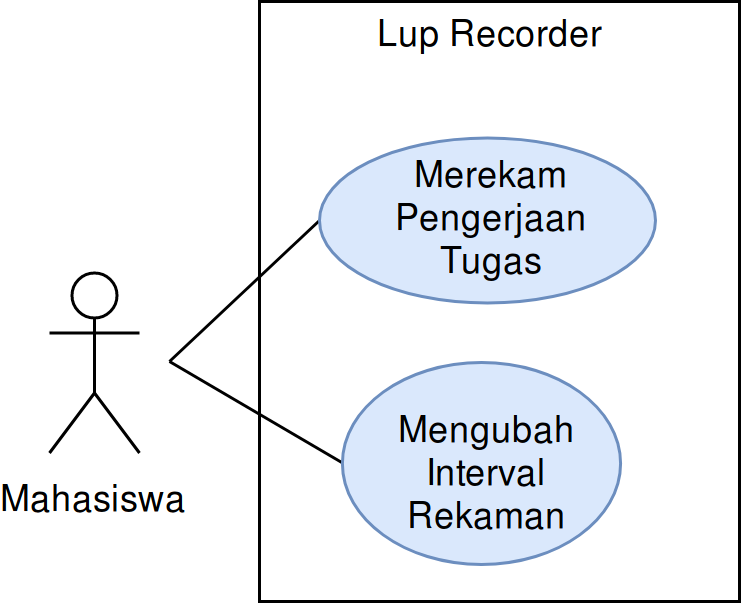
\includegraphics[width=.4\linewidth]{img/use-case/ucd-lupr-v3}
  \caption{\emph{Use case diagram} \emph{Lup Recorder}}\label{fig:ucd-lupr}
\end{figure}

\begin{figure}[H]
  \centering
  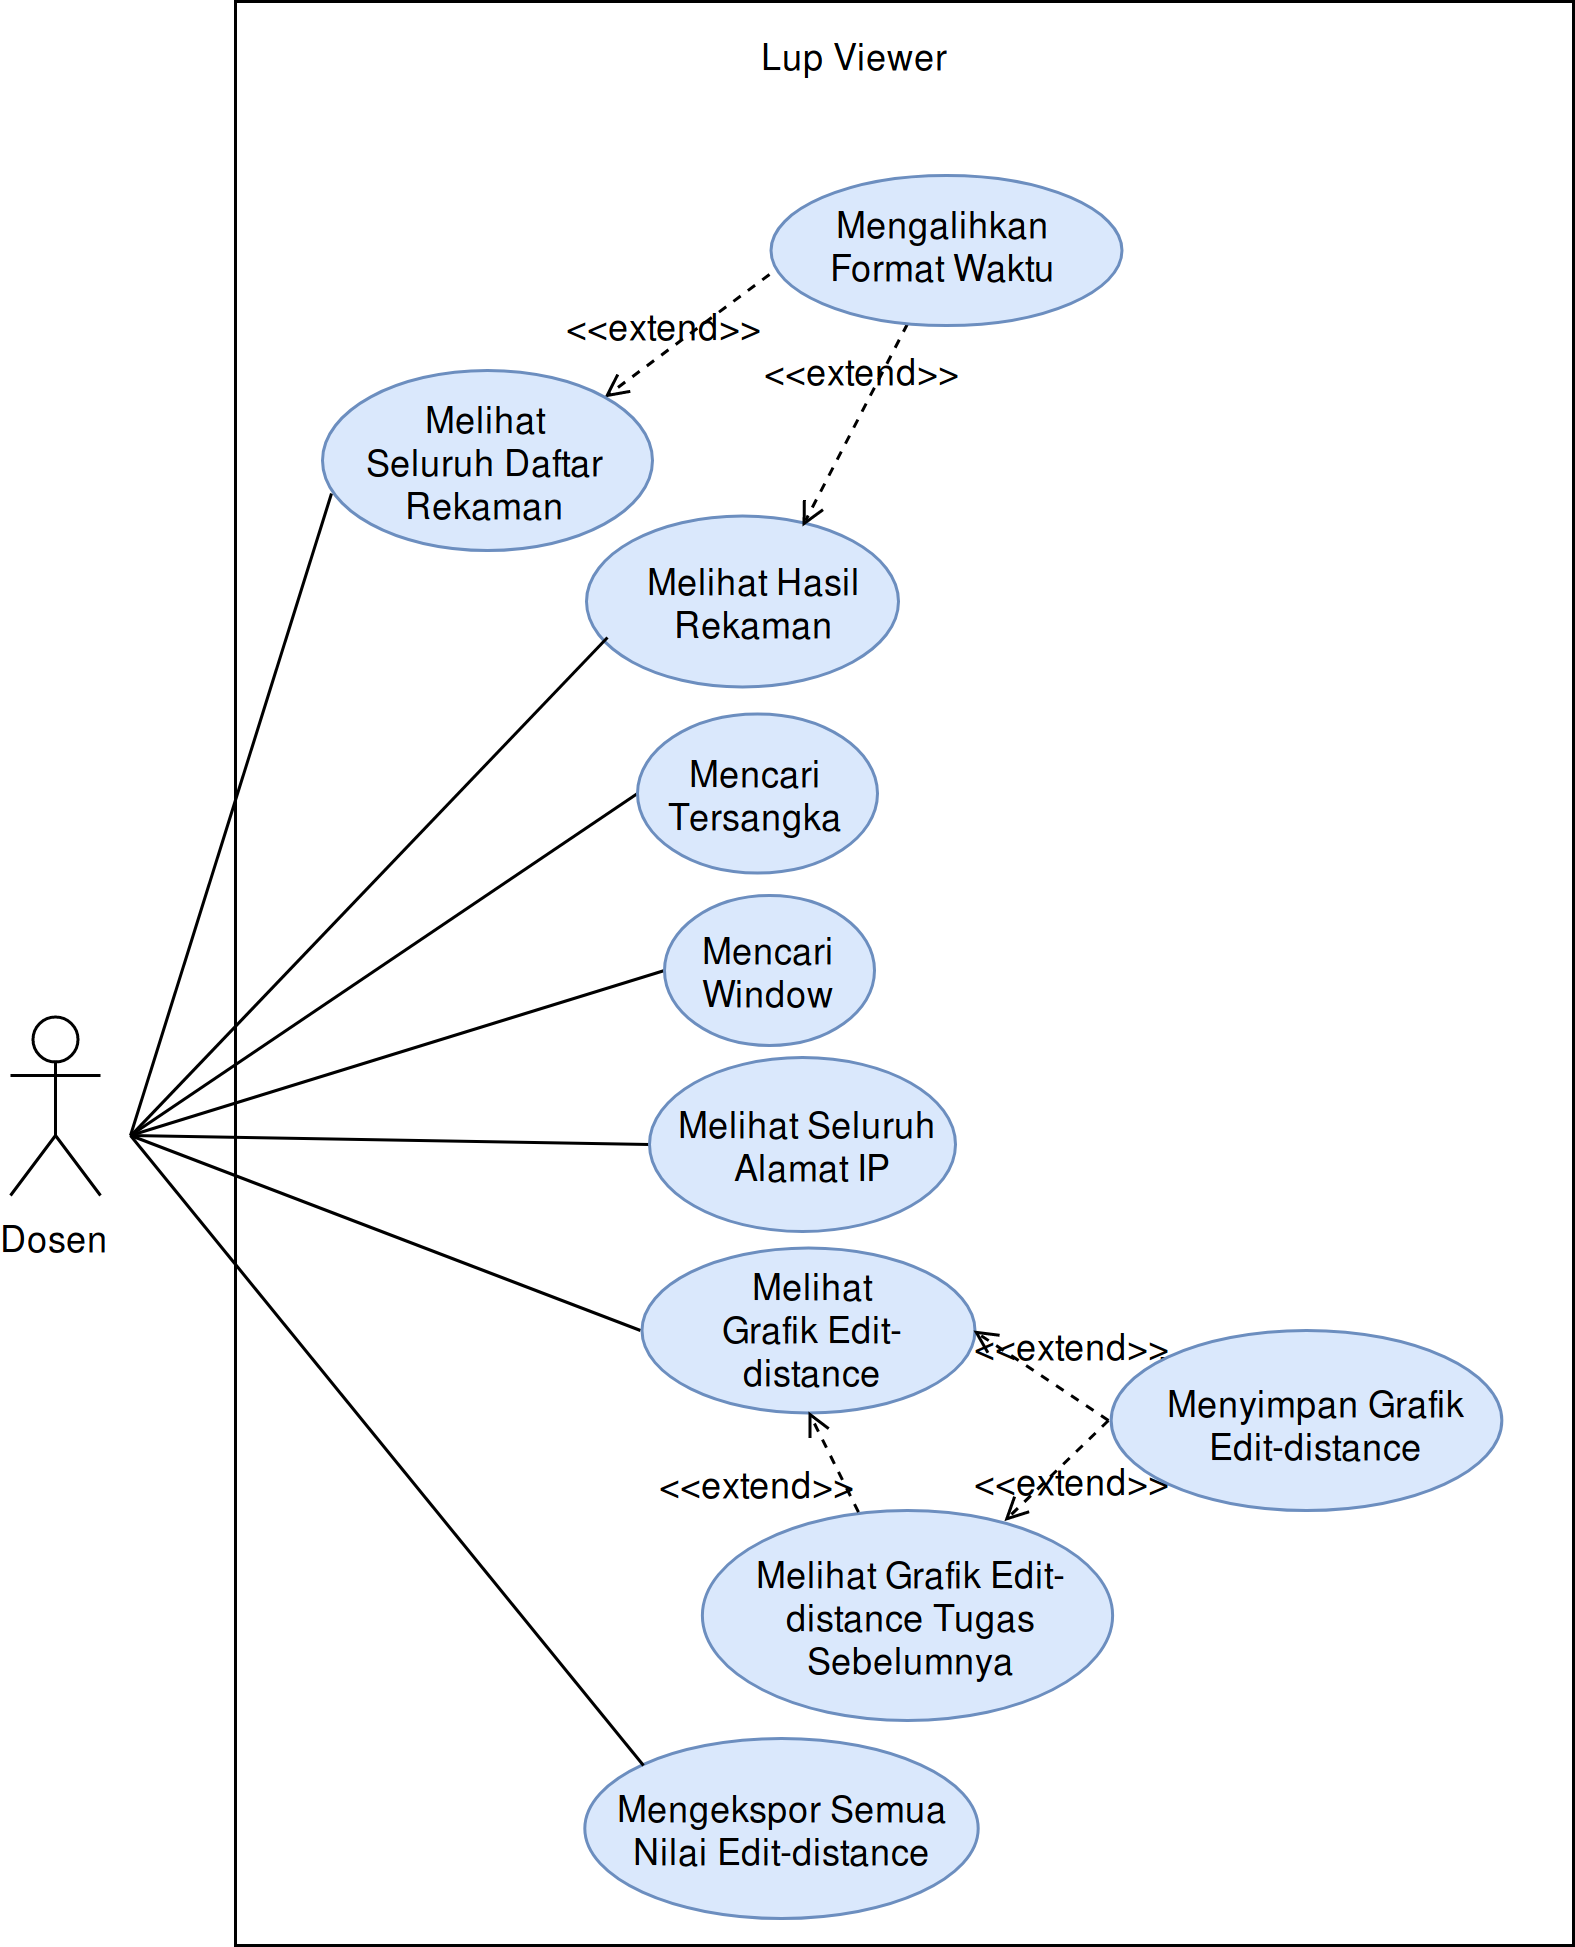
\includegraphics[width=.8\linewidth]{img/use-case/ucd-lupv-v3_1}
  \caption{\emph{Use case diagram} \emph{Lup Viewer}}\label{fig:ucd-lupv}
\end{figure}
\newpage % manual-adj

\subsection{\emph{Use Case Scenario}}


\emph{Use case scenario} digunakan untuk menjelaskan skenario interaksi antar
aktor dan sistem secara tekstual dengan detail. Dalam setiap \emph{use case
  scenario} dipaparkan \emph{objective} atau tujuan \emph{use case},
aktor yang terlibat, kondisi sebelumnya yang harus dipenuhi
\emph{pre-condition}, alur utama \emph{main flow}, alur alternatif
\emph{alternative flow}, dan kondisi setelah \emph{use case}
dijalankan \emph{post-condition}. \emph{Use case scenario} untuk
sistem \emph{Lup Recorder} dipaparkan pada
Tabel~\ref{tab:uc-merekam-tugas} hingga
Tabel~\ref{tab:uc-rubah-interval}, dan \emph{use case scenario} sistem
\emph{Lup Viewer} dipaparkan pada Tabel~\ref{tab:uc-seluruh-rekaman}
hingga~\ref{tab:uc-mengalihkan-waktu}.

\begin{longtable}{|L{3cm}|L{9cm}|}
  \caption{\emph{Use case scenario} untuk Merekam Pengerjaan Tugas}\label{tab:uc-merekam-tugas}\\
  \hline
  \multicolumn{2}{|L{12.5cm}|}{\emph{Flow of events} untuk Merekam Pengerjaan Tugas}\\\hline
  \textbf{Kode Kebutuhan} & LUPR-F-01 \\\hline
  %
  \textbf{\emph{Objective}} & Mahasiswa dapat merekam pengerjaan tugas.\\\hline
  %
  \textbf{\emph{Actor}} & Mahasiswa \\\hline
  %
  \textbf{\emph{Pre-condition}} & Tampilan utama sistem \emph{Lup Recorder} sudah tersedia. \\\hline
  %
  \textbf{\emph{Main flow}} & 1. Mahasiswa memilih tombol ``\emph{Start Recording}'' untuk mulai merekam
                              pengerjaan tugas. \newline
                              2. Sistem menampilkan dialog pemilihan letak direktori tugas. Pada dialog tersedia
                              tombol ``\emph{Choose}'' dan ``\emph{Cancel}''. \newline
                              3. Mahasiswa memilih letak direktori tugas dan memilih tombol ``\emph{Choose}''. \newline
                              4. Sistem menjalankan perekaman pengerjaan tugas dengan data yang
                              direkam meliputi berkas tugas, alamat \emph{IP}, seluruh \emph{window}, \emph{window}
                              yang aktif, nama \emph{login}, dan nama piranti.\newline
                              5. Sistem menampilkan pesan notifikasi ``\emph{Lup is recording}''
                              menandakan bahwa perekaman sudah dijalankan.\\\hline
  %
  \textbf{\emph{Alternative flows}} & 1.1 Sistem berhenti dan keluar jika mahasiswa memilih tombol
                                      ``\emph{Stop and Quit}''.\newline
                                      2.1 Sistem menutup dialog jika mahasiswa memilih tombol ``\emph{Cancel}''.\\\hline
  %
  \textbf{\emph{Post-condition}} & Pengerjaan tugas direkam oleh sistem.\\\hline
\end{longtable}
\newpage % manual-adj
\begin{longtable}{|L{3cm}|L{9cm}|}
  \caption{\emph{Use case scenario} untuk Mengubah Interval Rekaman}\label{tab:uc-rubah-interval} \\
  \hline
  \multicolumn{2}{|L{12.5cm}|}{\emph{Flow of events} untuk Mengubah Interval Rekaman}\\\hline
  \textbf{Kode Kebutuhan} & LUPR-F-02 \\\hline
  %
  \textbf{\emph{Objective}} & Mahasiswa dapat mengubah interval rekaman. \\\hline
  %
  \textbf{\emph{Actor}} & Mahasiswa \\\hline
  %
  \textbf{\emph{Pre-condition}} & Perekaman tugas sudah dijalankan. \\\hline
  %
  \textbf{\emph{Main flow}} & 1. Mahasiswa memilih tombol ``\emph{Set Interval}''. \newline
                              2. Sistem menampilkan dialog interval yang terdiri dari kolom nilai
                              interval. Pada dialog interval tersedia tombol ``\emph{Apply}'' dan ``\emph{Cancel}''. \newline
                              3. Mahasiswa memberikan nilai bilangan bulat diatas 0 pada kolom interval. \newline
                              4. Mahasiswa memilih tombol ``\emph{Apply}'' pada kolom interval. \newline
                              5. Sistem melakukan validasi nilai interval dan mengubah nilai interval rekaman.\newline
                              6. Sistem menampilkan pesan notifikasi ``\emph{Interval changed to
                              <<nilai interval>>}'' menandakan bahwa nilai interval berhasil dirubah.\\\hline
                              %
  \textbf{\emph{Alternative flows}} & 5.1 Apabila kolom bernilai selain bilangan bulat diatas 0, maka sistem
                                      menampilkan pesan peringatan ``\emph{Interval must higher than 0}''.\\\hline
  %
  \textbf{\emph{Post-condition}} & Nilai interval rekaman diubah oleh sistem. \\\hline
\end{longtable}

%% LUPR

\begin{longtable}{|L{3cm}|L{9cm}|}
  \caption{\emph{Use case scenario} untuk Melihat Seluruh Daftar Rekaman} \label{tab:uc-seluruh-rekaman}\\
  \hline
  \multicolumn{2}{|L{12.5cm}|}{\emph{Flow of events} untuk Melihat Seluruh Daftar Rekaman}\\\hline
  \textbf{Kode Kebutuhan} & LUPV-F-01 \\\hline
  %
  \textbf{\emph{Objective}} & Dosen dapat melihat seluruh daftar rekaman.\\\hline
  %
  \textbf{\emph{Actor}} & Dosen \\\hline
  %
  \textbf{\emph{Pre-condition}} & Tampilan utama sistem \emph{Lup Viewer} sudah tersedia.\\\hline
  %
  \textbf{\emph{Main flow}} & 1. Dosen memilih tombol ``\emph{Open Records}''. \newline
                              2. Sistem menampilkan dialog untuk memilih direktori rekaman yang akan dibuka.
                              Pada dialog tersebut terdapat tombol ``\emph{Choose}'' dan ``\emph{Cancel}''.\newline
                              3. Dosen memilih tombol ``\emph{Choose}''.\newline
                              4. Sistem melakukan validasi direktori rekaman dan menampilkan seluruh
                              daftar rekaman mahasiswa. Data yang ditampilkan meliputi nama, nim,
                              total rekaman, waktu rekaman awal, waktu rekaman akhir, dan durasi
                              pengerjaan.\\\hline
                              %
  \textbf{\emph{Alternative flows}} & 3.1 Apabila dosen memilih tombol ``\emph{Cancel}'', maka
                                      berkas rekaman tidak dibuka. \newline
                                      4.1 Apabila direktori tidak valid, yaitu tidak sesuai dengan
                                      spesifikasi kebutuhan LUPV-F-01-02 dan LUPV-F-01-03, maka sistem
                                      menampilkan pesan peringatan ``\emph{Not a valid Task
                                      directory (baris baru) Contains invalid Task: <<direktori yang tidak valid>>}''. \newline
                                      4.2 Perluasan ke \emph{use case} dengan kode kebutuhan LUPV-F-10.\\\hline
  %
  \textbf{\emph{Post-condition}} & Seluruh daftar rekaman ditampilkan oleh sistem. \\\hline
\end{longtable}

\begin{longtable}{|L{3cm}|L{9cm}|}
  \caption{\emph{Use case scenario} untuk Menampilkan Hasil Rekaman} \label{tab:uc-hasil-rekaman} \\
  \hline
  \multicolumn{2}{|L{12.5cm}|}{\emph{Flow of events} untuk Melihat Hasil Rekaman}\\\hline
  \textbf{Kode Kebutuhan} & LUPV-F-02 \\\hline
  %
  \textbf{\emph{Objective}} & Dosen dapat melihat hasil rekaman.\\\hline
  %
  \textbf{\emph{Actor}} & Dosen \\\hline
  %
  \textbf{\emph{Pre-condition}} & Tampilan seluruh daftar rekaman mahasiswa sudah tersedia. \\\hline
  %
  \textbf{\emph{Main flow}} & 1. Dosen memilih \emph{clickable} baris mahasiswa pada seluruh daftar rekaman.\newline
                              2. Sistem menampilkan \emph{clickable list} daftar rekaman. \newline
                              3. Dosen memilih \emph{clickable list} daftar rekaman. \newline
                              4. Sistem menampilkan rekaman alamat \emph{IP}, seluruh \emph{window},
                              \emph{window} yang aktif, nama \emph{login}, dan nama piranti. \newline
                              5. Dosen memilih nama berkas pada tombol \emph{combo box}
                              ``\emph{Filename}''. \newline
                              6. Sistem menampilkan hasil rekaman isi perubahan berkas. \newline
                              7. Dosen memilih tombol ``\emph{Line Insertion and Deletion}''.\newline
                              8. Sistem menampilkan jumlah baris yang dihapus dan jumlah baris yang
                              ditambah pada berkas.\newline
                              9. Dosen memilih tombol ``\emph{Show Mode}'' dan ``\emph{Diff Mode}''.\newline
                              10. Sistem menampilkan format perubahan berkas dengan mode \emph{show}
                              dan mode \emph{diff}. \\\hline
                              %
  \textbf{\emph{Alternative flows}} & 4.1 Perluasan ke \emph{use case} dengan kode kebutuhan
                                      LUPV-F-10. \newline
                                      6.1 Sistem menampilkan pesan informasi ``\emph{No file selected, please
                                      select one}'' jika tidak ada berkas tugas yang dipilih.\newline
                                      6.2 Sistem menampilkan pesan informasi ``\emph{No availiable record for
                                      «nama berkas» in this period}''  jika tidak ada perubahan tugas
                                      pada rekaman yang dipilih.\newline
                                      7.1 Sistem menampilkan pesan peringatan ``\emph{Please choose
                                      a file}'' jika tidak ada berkas yang dipilih.\\\hline
  %
  \textbf{\emph{Post-condition}} & Hasil rekaman ditampilkan oleh sistem. \\\hline
\end{longtable}

\begin{longtable}{|L{3cm}|L{9cm}|}
  \caption{\emph{Use case scenario} untuk Mencari Tersangka.} \label{tab:uc-search-suspect} \\
  \hline
  \multicolumn{2}{|L{12.5cm}|}{\emph{Flow of events} untuk Mencari Tersangka}\\\hline
  \textbf{Kode Kebutuhan} & LUPV-F-03 \\\hline
  %
  \textbf{\emph{Objective}} & Dosen dapat mencari tersangka. \\\hline
  %
  \textbf{\emph{Actor}} & Dosen \\\hline
  %
  \textbf{\emph{Pre-condition}} & Tampilan pencarian tersangka sudah tersedia. \\\hline
  %
  \textbf{\emph{Main flow}} & 1. Dosen memilih nama berkas dari tombol \emph{combo box}
                              ``\emph{Filename}'' dan mengisi nilai ``\emph{Line Insertion
                              Limit}''. \newline
                              2. Dosen memilih tombol ``\emph{Search}'' untuk menjalankan pencarian.\newline
                              3. Sistem melakukan validasi nilai ``\emph{Line Insertion Limit}''
                              dan menampilkan hasil pencarian tersangka.\\\hline
                              %
  \textbf{\emph{Alternative flows}} & 3.1 Sistem menampilkan pesan peringatan ``\emph{Please set limit
                                      higher than 0 (baris baru) Above 10 is recommended}'' apabila nilai pada
                                      kolom \emph{insertion} bernilai selain bilangan bulat di
                                      atas 0. \newline
                                      3.2 Sistem menampilkan pesan informasi ``\emph{No suspect found,
                                      for <<limit>> insertion limit}'' jika tidak ada tersangka yang
                                      ditemukan. \newline
                                      3.3 Sistem menampilkan pesan peringatan ``\emph{Please select a
                                      file}'' apabila tidak ada berkas tugas yang
                                      dipilih. \\\hline
  %
  \textbf{\emph{Post-condition}} & Hasil pencarian tersangka ditampilkan oleh sistem.\\\hline
\end{longtable}


\begin{longtable}{|L{3cm}|L{9cm}|}
  \caption{\emph{Use case scenario} untuk Mencari \emph{Window}} \label{tab:uc-search-window} \\
  \hline
  \multicolumn{2}{|L{12.5cm}|}{\emph{Flow of events} untuk Mencari \emph{Window}}\\\hline
  \textbf{Kode Kebutuhan} & LUPV-F-04 \\\hline
  %
  \textbf{\emph{Objective}} & Dosen dapat mencari \emph{window}. \\\hline
  %
  \textbf{\emph{Actor}} & Dosen \\\hline
  %
  \textbf{\emph{Pre-condition}} & Tampilan pencarian \emph{window} telah tersedia. \\\hline
  %
  \textbf{\emph{Main flow}} & 1. Dosen mengisi kolom ``\emph{Window Name}''. \newline
                              2. Dosen memilih tombol ``\emph{Search}'' untuk menjalankan pencarian.\newline
                              3. Sistem melakukan validasi nilai kolom ``\emph{Window Name}''
                              dan menampilkan hasil pencarian \emph{window}.\\\hline
                              %
  \textbf{\emph{Alternative flows}} & 3.1 Sistem menampilkan pesan informasi ``\emph{No window name for
                                      <<nama window>> found}'' jika tidak ada \emph{window} yang ditemukan. \newline
                                      3.1 Sistem menampilkan pesan peringatan ``\emph{Please
                                      supply the window name}'' apabila kolom
                                      ``\emph{Window Name}'' kosong. \\\hline
  %
  \textbf{\emph{Post-condition}} & Hasil pencarian \emph{window} ditampilkan oleh sistem.\\\hline
\end{longtable}


\begin{longtable}{|L{3cm}|L{9cm}|}
  \caption{\emph{Use case scenario} untuk Menampilkan Seluruh Alamat \emph{IP}} \label{tab:uc-show-ips} \\
  \hline
  \multicolumn{2}{|L{12.5cm}|}{\emph{Flow of events} untuk Melihat Seluruh Alamat \emph{IP}}\\\hline
  \textbf{Kode Kebutuhan} & LUPV-F-05 \\\hline
  %
  \textbf{\emph{Objective}} & Dosen dapat melihat seluruh alamat \emph{IP}. \\\hline
  %
  \textbf{\emph{Actor}} & Dosen \\\hline
  %
  \textbf{\emph{Pre-condition}} & Tampilan untuk melihat seluruh alamat \emph{IP} telah tersedia. \\\hline
  %
  \textbf{\emph{Main flow}} & 1. Dosen memilih tombol ``\emph{Show all IP addresses}''. \newline
                              2. Sistem menampilkan seluruh alamat \emph{IP}.\\\hline
                              %
  \textbf{\emph{Alternative flows}} & - \\\hline
  %
  \textbf{\emph{Post-condition}} & Seluruh alamat \emph{IP} ditampilkan oleh sistem\\\hline
\end{longtable}


\begin{longtable}{|L{3cm}|L{9cm}|}
  \caption{\emph{Use case scenario} untuk Melihat Grafik \emph{Edit-distance}.} \label{tab:uc-edit-distance} \\
  \hline
  \multicolumn{2}{|L{12.5cm}|}{\emph{Flow of events} untuk Melihat Grafik \emph{Edit-distance}}\\\hline
  \textbf{Kode Kebutuhan} & LUPV-F-06 \\\hline
  %
  \textbf{\emph{Objective}} & Dosen dapat melihat grafik \emph{edit-distance}. \\\hline
  %
  \textbf{\emph{Actor}} & Dosen \\\hline
  %
  \textbf{\emph{Pre-condition}} & Tampilan untuk melihat grafik \emph{edit-distance} telah tersedia. \\\hline
  %
  \textbf{\emph{Main flow}} & 1. Dosen memilih mahasiswa dari tombol \emph{combo box} ``\emph{Current
                              Student}'' dan memilih berkas dari tombol \emph{combo box}
                              ``\emph{Filename}''. \newline
                              2. Dosen memilih tombol ``\emph{Show Mode}''.\newline
                              3. Sistem melakukan validasi nilai tombol \emph{combo box}
                              ``\emph{Current Student}'' dan ``\emph{Filename}'', kemudian menampilkan
                              grafik  \emph{edit distance}.\\\hline
                              %
  \textbf{\emph{Alternative flows}} & 1.2 Perluasan ke \emph{use case} dengan kode kebutuhan
                                      LUPV-F-07 dan LUPV-F-08. \newline
                                      2.1  Sistem menampilkan pesan peringatan ``\emph{Please fill
                                      one of the pairs}'' jika salah satu atau
                                      kedua \emph{combo box} ``\emph{Filename}'' dan ``\emph{Current
                                      Student}'' tidak diisi. \\\hline

  %
  \textbf{\emph{Post-condition}} & Grafik \emph{edit distance} ditampilkan oleh sistem.\\\hline
\end{longtable}

\begin{longtable}{|L{3cm}|L{9cm}|}
  \caption{\emph{Use case scenario} untuk Melihat Grafik \emph{Edit-distance} Tugas Sebelumnya} \label{tab:uc-prev-edit-distance} \\
  \hline
  \multicolumn{2}{|L{12.5cm}|}{\emph{Flow of events} untuk Melihat Grafik \emph{Edit-distance} Tugas Sebelumnya}\\\hline
  \textbf{Kode Kebutuhan} & LUPV-F-07 \\\hline
  %
  \textbf{\emph{Objective}} & Dosen dapat melihat grafik \emph{edit-distance} tugas sebelumnya. \\\hline
  %
  \textbf{\emph{Actor}} & Dosen \\\hline
  %
  \textbf{\emph{Pre-condition}} & Tampilan untuk melihat grafik \emph{edit-distance} telah tersedia. \\\hline
  %
  \textbf{\emph{Main flow}} & 1. Dosen memilih tombol ``\emph{Load Edit-distance}''.\newline
                              2. Sistem menampilkan dialog untuk memilih berkas \emph{edit-distance}
                              tugas sebelumnya. Dialog memiliki tombol ``\emph{Open}'' dan
                              ``\emph{Cancel}''.\newline
                              3. Dosen memilih berkas dan memilih tombol ``\emph{Open}''.\newline
                              4. Sistem membaca berkas \emph{edit-distance} tugas sebelumnya.\newline
                              5. Dosen memilih mahasiswa dari tombol \emph{combo box} ``\emph{Previous
                              Student}'' dan memilih berkas dari tombol \emph{combo box}
                              ``\emph{Filename}''. \newline
                              6. Dosen memilih tombol ``\emph{Show Mode}''.\newline
                              7. Sistem melakukan validasi nilai tombol \emph{combo box}
                              ``\emph{Previous Student}'' dan ``\emph{Filename}'', kemudian
                              menampilkan grafik  \emph{edit distance} tugas sebelumnya.\\\hline
                              %
  \textbf{\emph{Alternative flows}} & 3.1 Sistem tidak membaca berkas jika dosen memilih tombol
                                      ``\emph{Cancel}''.\newline
                                      5.1 Sistem menampilkan pesan peringatan ``\emph{Please load
                                      edit-distance file first}'' jika dosen belum
                                      membuka berkas \emph{edit-distance} tugas sebelumnya. \newline
                                      5.2  Sistem menampilkan pesan peringatan ``\emph{Please fill
                                      one of the pairs}'' jika salah satu atau
                                      kedua \emph{combo box} ``\emph{Filename}'' dan ``\emph{Previous
                                      Student}'' belum dipilih.\newline
                                      6.1 Perluasan ke \emph{use case} dengan kode kebutuhan LUPV-F-08.\\\hline
  %
  \textbf{\emph{Post-condition}} & Grafik \emph{edit distance} tugas sebelumnya ditampilkan oleh sistem.\\\hline
\end{longtable}


\begin{longtable}{|L{3cm}|L{9cm}|}
  \caption{\emph{Use case scenario} untuk Menyimpan Grafik \emph{Edit-distance}}. \label{tab:uc-save-graph} \\
  \hline
  \multicolumn{2}{|L{12.5cm}|}{\emph{Flow of events} untuk Menyimpan Grafik \emph{Edit-distance}}\\\hline
  \textbf{Kode Kebutuhan} & LUPV-F-08 \\\hline
  %
  \textbf{\emph{Objective}} & Dosen dapat menyimpan grafik \emph{edit-distance}. \\\hline
  %
  \textbf{\emph{Actor}} & Dosen \\\hline
  %
  \textbf{\emph{Pre-condition}} &  Grafik \emph{edit-distance} telah tersedia. \\\hline
  %
  \textbf{\emph{Main flow}} & 1. Dosen memilih tombol ``\emph{Save Graph}''.\newline
                              2. Sistem menyimpan grafik pada direktori ``\emph{lupv-notes}'' pada
                              direktori tugas. \newline
                              3. Sistem menampilkan pesan informasi ``\emph{Graph saved to
                              <<lokasi berkas>>}'' menandakan bahwa grafik telah disimpan. \\\hline
                              %
  \textbf{\emph{Alternative flows}} & -\\\hline
  %
  \textbf{\emph{Post-condition}} & Grafik \emph{edit distance} disimpan oleh sistem.\\\hline
\end{longtable}

\begin{longtable}{|L{3cm}|L{9cm}|}
  \caption{\emph{Use case scenario} untuk Mengekspor Semua Nilai \emph{Edit-distance}}. \label{tab:uc-export-ed} \\
  \hline
  \multicolumn{2}{|L{12.5cm}|}{\emph{Flow of events} untuk Mengekspor Semua Nilai \emph{Edit-distance}}\\\hline
  \textbf{Kode Kebutuhan} & LUPV-F-09 \\\hline
  %
  \textbf{\emph{Objective}} & Dosen dapat mengekspor semua nilai \emph{edit-distance}. \\\hline
  %
  \textbf{\emph{Actor}} & Dosen \\\hline
  %
  \textbf{\emph{Pre-condition}} &  Tampilan seluruh daftar rekaman mahasiswa telah tersedia. \\\hline
  %
  \textbf{\emph{Main flow}} & 1. Dosen memilih tombol ``\emph{Export Edit-distance}''.\newline
                              2. Sistem menampilkan dialog pemilihan berkas yang akan di
                              ekspor. Pada dialog tersedia tombol ``\emph{Export}''
                              dan ``\emph{Cancel}''.\newline
                              3. Dosen memilih tombol ``\emph{Export}''.\newline
                              4. Sistem mengekspor semua nilai \emph{edit-distance} pada berkas
                              yang dipilih dan menyimpan hasil ekspor dengan nama
                              ``<<namatugas>>-editdistance.lup''. \newline
                              5. Sistem menampilkan pesan informasi ``\emph{Edit-distance exported
                              to <<lokasi berkas>>}'' menandakan bahwa semua nilai
                              \emph{edit-distance} telah diekspor. \\\hline
                              %
  \textbf{\emph{Alternative flows}} & 3.1 Apabila dosen memilih tombol ``\emph{Cancel}'', maka
                                      sistem menutup dialog pemilihan berkas dan
                                      nilai \emph{edit-distance} tidak diekspor.\\\hline
  %
  \textbf{\emph{Post-condition}} &  Semua nilai \emph{edit-distance} diekspor oleh sistem.\\\hline
\end{longtable}

\begin{longtable}{|L{3cm}|L{9cm}|}
  \caption{\emph{Use case scenario} untuk Mengalihkan Format Waktu}. \label{tab:uc-mengalihkan-waktu} \\
  \hline
  \multicolumn{2}{|L{12.5cm}|}{\emph{Flow of events} untuk Mengalihkan Format Waktu}\\\hline
  \textbf{Kode Kebutuhan} & LUPV-F-10 \\\hline
  %
  \textbf{\emph{Objective}} & Dosen dapat mengalihkan format waktu. \\\hline
  %
  \textbf{\emph{Actor}} & Dosen \\\hline
  %
  \textbf{\emph{Pre-condition}} &  Tampilan waktu rekaman telah tersedia. \\\hline
  %
  \textbf{\emph{Main flow}} & 1. Dosen memilih tombol ``\emph{Real DateTime}'' dan ``\emph{Relative
                              DateTime}''.\newline
                              2. Sistem mengalihkan format waktu. Format bentuk ``<<nama pendek
                              hari, tanggal bulan tahun, jam:menit:detik>>'' untuk format
                              \emph{real} dan ``<<x \emph{hours ago}>>'' untuk format
                              \emph{relative}.\\\hline
  %
  \textbf{\emph{Alternative flows}} & - \\\hline
  %
  \textbf{\emph{Post-condition}} & Format waktu dialihkan oleh sistem.\\\hline
\end{longtable}

%%% Local Variables:
%%% coding: utf-8
%%% mode: latex
%%% TeX-engine: xetex
%%% TeX-master: "skripsi"
%%% ispell-local-dictionary: "id"
%%% End:
